\documentclass[tikz,border=10pt]{standalone}
\usepackage{amsmath,amssymb}
\usepackage{tikz}
\usetikzlibrary{arrows.meta,calc,positioning,fit,backgrounds}

\definecolor{navy}{HTML}{1B365D}
\definecolor{steelblue}{HTML}{2471A3}
\definecolor{softblue}{HTML}{D4E6F1}
\definecolor{teal}{HTML}{0E6251}
\definecolor{softteal}{HTML}{D1F2EB}
\definecolor{amber}{HTML}{B9770E}
\definecolor{softamber}{HTML}{FCF3CF}
\definecolor{crimson}{HTML}{922B21}
\definecolor{softred}{HTML}{FADBD8}
\definecolor{slate}{HTML}{566573}

\begin{document}
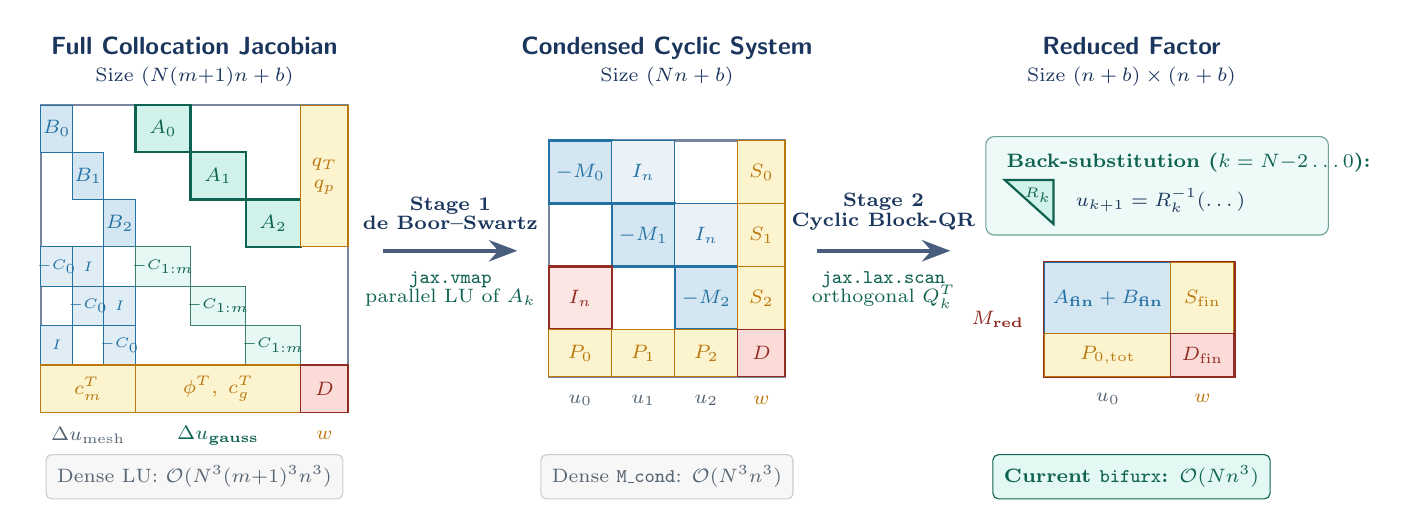
\begin{tikzpicture}[
    >=Stealth,
    font=\sffamily\footnotesize,
    blk/.style={draw=navy!80, line width=0.7pt},
    arrowstage/.style={->, line width=1.6pt, color=navy!80},
]

% ========================
% PANEL 1: Full Collocation Jacobian
% ========================
\begin{scope}[shift={(0,0)}]
    \node[font=\sffamily\bfseries\small, navy, align=center] at (1.95, 4.45)
        {Full Collocation Jacobian\\[-1pt]\normalfont\scriptsize Size $(N(m{+}1)n + b)$};

    % Outer frame
    \draw[thick, navy!60] (0,0) rectangle (3.9, 3.9);

    % Top-left: u_mesh (0..1.2) x coll (2.1..3.9) -> B_k blocks
    \foreach \k in {0,1,2} {
        \fill[softblue, draw=steelblue] ({0.4*\k}, {3.3 - 0.6*\k}) rectangle ({0.4*\k + 0.4}, {3.9 - 0.6*\k});
        \node[steelblue, font=\scriptsize] at ({0.4*\k + 0.2}, {3.6 - 0.6*\k}) {$B_{\k}$};
    }

    % Top-mid: u_gauss (1.2..3.3) x coll (2.1..3.9) -> A_k blocks (parallel LU!)
    \foreach \k in {0,1,2} {
        \fill[softteal, draw=teal, thick] ({1.2 + 0.7*\k}, {3.3 - 0.6*\k}) rectangle ({1.2 + 0.7*\k + 0.7}, {3.9 - 0.6*\k});
        \node[teal, font=\scriptsize\bfseries] at ({1.2 + 0.7*\k + 0.35}, {3.6 - 0.6*\k}) {$A_{\k}$};
    }

    % Top-right: border cols q_T, q_p (3.3..3.9) x coll (2.1..3.9)
    \fill[softamber, draw=amber] (3.3, 2.1) rectangle (3.9, 3.9);
    \node[amber, font=\scriptsize, align=center] at (3.6, 3.0) {$q_T$\\$q_p$};

    % Mid-left: continuity u_mesh (0..1.2) x cont (0.6..2.1)
    \fill[softblue!70, draw=steelblue] (0, 1.6) rectangle (0.4, 2.1);
    \fill[softblue!70, draw=steelblue] (0.4, 1.6) rectangle (0.8, 2.1);
    \fill[softblue!70, draw=steelblue] (0.4, 1.1) rectangle (0.8, 1.6);
    \fill[softblue!70, draw=steelblue] (0.8, 1.1) rectangle (1.2, 1.6);
    \fill[softblue!70, draw=steelblue] (0.8, 0.6) rectangle (1.2, 1.1);
    \fill[softblue!70, draw=steelblue] (0.0, 0.6) rectangle (0.4, 1.1);
    \node[steelblue, font=\tiny] at (0.2, 1.85) {$-C_0$};
    \node[steelblue, font=\tiny] at (0.6, 1.85) {$I$};
    \node[steelblue, font=\tiny] at (0.6, 1.35) {$-C_0$};
    \node[steelblue, font=\tiny] at (1.0, 1.35) {$I$};
    \node[steelblue, font=\tiny] at (1.0, 0.85) {$-C_0$};
    \node[steelblue, font=\tiny] at (0.2, 0.85) {$I$};

    % Mid-mid: continuity u_gauss (1.2..3.3) x cont (0.6..2.1) -> -C_{1:m}
    \foreach \k in {0,1,2} {
        \fill[softteal!55, draw=teal!80] ({1.2 + 0.7*\k}, {1.6 - 0.5*\k}) rectangle ({1.2 + 0.7*\k + 0.7}, {2.1 - 0.5*\k});
        \node[teal, font=\tiny] at ({1.2 + 0.7*\k + 0.35}, {1.85 - 0.5*\k}) {$-C_{1:m}$};
    }

    % Bottom row: phase + arclength border (0..3.9) x (0..0.6)
    \fill[softamber, draw=amber] (0, 0) rectangle (1.2, 0.6);
    \node[amber, font=\scriptsize] at (0.6, 0.3) {$c_m^T$};
    \fill[softamber, draw=amber] (1.2, 0) rectangle (3.3, 0.6);
    \node[amber, font=\scriptsize] at (2.25, 0.3) {$\phi^T, \; c_g^T$};
    \fill[softred, draw=crimson] (3.3, 0) rectangle (3.9, 0.6);
    \node[crimson, font=\scriptsize] at (3.6, 0.3) {$D$};

    % Column group labels at bottom
    \node[slate, font=\scriptsize] at (0.6, -0.30) {$\Delta u_{\text{mesh}}$};
    \node[teal, font=\scriptsize\bfseries] at (2.25, -0.30) {$\Delta u_{\text{gauss}}$};
    \node[amber, font=\scriptsize] at (3.6, -0.30) {$w$};

    % Cost badge
    \node[draw=black!20, fill=black!3, rounded corners=2pt, font=\scriptsize, text=slate, inner sep=4pt]
        at (1.95, -0.82) {Dense LU: $\mathcal{O}(N^3(m{+}1)^3 n^3)$};
\end{scope}

% Arrow Stage 1
\draw[arrowstage] (4.35, 2.05) -- (6.05, 2.05);
\node[navy, font=\scriptsize\bfseries, align=center, above=4pt] at (5.20, 2.05)
    {Stage 1\\[-1pt]de Boor--Swartz};
\node[teal, font=\scriptsize, align=center, below=4pt] at (5.20, 2.05)
    {\texttt{jax.vmap}\\[-1pt]parallel LU of $A_k$};

% ========================
% PANEL 2: Condensed Cyclic Block-Bidiagonal + Border
% ========================
\begin{scope}[shift={(6.45, 0.45)}]
    \node[font=\sffamily\bfseries\small, navy, align=center] at (1.5, 4.0)
        {Condensed Cyclic System\\[-1pt]\normalfont\scriptsize Size $(Nn + b)$};

    \draw[thick, navy!60] (0,0) rectangle (3.0, 3.0);

    % 3x3 cyclic block-bidiagonal (0..2.4) x (0.6..3.0), each block 0.8x0.8
    % Row 0: -M_0, I, 0
    \fill[softblue, draw=steelblue, thick] (0.0, 2.2) rectangle (0.8, 3.0);
    \node[steelblue, font=\scriptsize\bfseries] at (0.4, 2.6) {$-M_0$};
    \fill[softblue!50, draw=steelblue] (0.8, 2.2) rectangle (1.6, 3.0);
    \node[steelblue, font=\scriptsize] at (1.2, 2.6) {$I_n$};

    % Row 1: 0, -M_1, I
    \fill[softblue, draw=steelblue, thick] (0.8, 1.4) rectangle (1.6, 2.2);
    \node[steelblue, font=\scriptsize\bfseries] at (1.2, 1.8) {$-M_1$};
    \fill[softblue!50, draw=steelblue] (1.6, 1.4) rectangle (2.4, 2.2);
    \node[steelblue, font=\scriptsize] at (2.0, 1.8) {$I_n$};

    % Row 2: I, 0, -M_2 (cyclic wrap-around!)
    \fill[softred!70, draw=crimson, thick] (0.0, 0.6) rectangle (0.8, 1.4);
    \node[crimson, font=\scriptsize\bfseries] at (0.4, 1.0) {$I_n$};
    \fill[softblue, draw=steelblue, thick] (1.6, 0.6) rectangle (2.4, 1.4);
    \node[steelblue, font=\scriptsize\bfseries] at (2.0, 1.0) {$-M_2$};

    % Right border column S_k (2.4..3.0) x (0.6..3.0)
    \foreach \k/\yy in {0/2.2, 1/1.4, 2/0.6} {
        \fill[softamber, draw=amber] (2.4, \yy) rectangle (3.0, {\yy+0.8});
        \node[amber, font=\scriptsize] at (2.7, {\yy+0.4}) {$S_{\k}$};
    }

    % Bottom border row P_k (0..2.4) x (0..0.6)
    \foreach \k/\xx in {0/0.0, 1/0.8, 2/1.6} {
        \fill[softamber, draw=amber] (\xx, 0.0) rectangle ({\xx+0.8}, 0.6);
        \node[amber, font=\scriptsize] at ({\xx+0.4}, 0.3) {$P_{\k}$};
    }
    \fill[softred, draw=crimson] (2.4, 0.0) rectangle (3.0, 0.6);
    \node[crimson, font=\scriptsize] at (2.7, 0.3) {$D$};

    % Column labels
    \node[slate, font=\scriptsize] at (0.4, -0.30) {$u_0$};
    \node[slate, font=\scriptsize] at (1.2, -0.30) {$u_1$};
    \node[slate, font=\scriptsize] at (2.0, -0.30) {$u_2$};
    \node[amber, font=\scriptsize] at (2.7, -0.30) {$w$};

    % Cost badge
    \node[draw=black!20, fill=black!3, rounded corners=2pt, font=\scriptsize, text=slate, inner sep=4pt]
        at (1.5, -1.27) {Dense \texttt{M\_cond}: $\mathcal{O}(N^3 n^3)$};
\end{scope}

% Arrow Stage 2
\draw[arrowstage] (9.85, 2.05) -- (11.55, 2.05);
\node[navy, font=\scriptsize\bfseries, align=center, above=4pt] at (10.70, 2.05)
    {Stage 2\\[-1pt]Cyclic Block-QR};
\node[teal, font=\scriptsize, align=center, below=4pt] at (10.70, 2.05)
    {\texttt{jax.lax.scan}\\[-1pt]orthogonal $Q_k^T$};

% ========================
% PANEL 3: Reduced System after Orthogonal Block-QR
% ========================
\begin{scope}[shift={(12.0, 0.45)}]
    \node[font=\sffamily\bfseries\small, navy, align=center] at (1.85, 4.0)
        {Reduced Factor\\[-1pt]\normalfont\scriptsize Size $(n + b) \times (n + b)$};

    % Clean triangular R_k back-substitution box
    \draw[draw=teal!60, fill=softteal!40, rounded corners=3pt] (0.0, 1.80) rectangle (4.35, 3.05);
    \node[teal, font=\scriptsize\bfseries, anchor=north west] at (0.14, 2.97)
        {Back-substitution ($k = N{-}2 \dots 0$):};
    \fill[softteal, draw=teal, thick] (0.24, 2.50) -- (0.86, 2.50) -- (0.86, 1.94) -- cycle;
    \node[teal, font=\tiny\bfseries] at (0.66, 2.31) {$R_k$};
    \node[navy, font=\scriptsize, anchor=west] at (1.02, 2.24) {$u_{k+1} = R_k^{-1}(\dots)$};

    % Tiny (n+b) x (n+b) M_red block
    \begin{scope}[shift={(0.75, 0.0)}]
        \draw[very thick, crimson] (0,0) rectangle (2.40, 1.45);
        \fill[softblue, draw=steelblue] (0, 0.55) rectangle (1.60, 1.45);
        \node[steelblue, font=\scriptsize\bfseries] at (0.80, 1.00) {$A_{\text{fin}} + B_{\text{fin}}$};
        \fill[softamber, draw=amber] (1.60, 0.55) rectangle (2.40, 1.45);
        \node[amber, font=\scriptsize] at (2.00, 1.00) {$S_{\text{fin}}$};
        \fill[softamber, draw=amber] (0, 0.0) rectangle (1.60, 0.55);
        \node[amber, font=\scriptsize] at (0.80, 0.275) {$P_{0,\text{tot}}$};
        \fill[softred, draw=crimson] (1.60, 0.0) rectangle (2.40, 0.55);
        \node[crimson, font=\scriptsize] at (2.00, 0.275) {$D_{\text{fin}}$};
        \node[crimson, font=\scriptsize\bfseries, left=4pt] at (0, 0.725) {$M_{\text{red}}$};
        \node[slate, font=\scriptsize] at (0.80, -0.28) {$u_0$};
        \node[amber, font=\scriptsize] at (2.00, -0.28) {$w$};
    \end{scope}

    % Cost badge (highlighted!)
    \node[draw=teal, fill=softteal!60, rounded corners=2pt, font=\scriptsize\bfseries, text=teal, inner sep=4pt]
        at (1.85, -1.27) {Current \texttt{bifurx}: $\mathcal{O}(N n^3)$};
\end{scope}

\end{tikzpicture}
\end{document}
